%
%  thesis.tex   2003.03.23  13:52:27   Mark D Senn <mds@purdue.edu>
%
%  This is the ``main file'' for a simple, example thesis.
%
%  To make the final copy of the thesis comment
%  out the \includeonly command below and type:
%      latex thesis
%      bibtex thesis
%      latex thesis
%      latex thesis
%
%  Regarding ``References'' below:
%      KEY  MEANING
%      PU   ``A Manual for the Preparation of Graduate Theses'',
%           The Graduate School, Purdue University, 1996.
%
%  MARKERS:
%    $+
%    $dpps:  dp -ps $f1
%    $gs:    gs $f1.ps
%    $latex: latex $f1
%    $-
%
%  HISTORY:
%    2003.03.13 Improved comments.
%               Added MARKERS section for Mark Senn.
%

  % See http://www.ecn.purdue.edu/ECN/Documents/tex/latex/puthesis
  % for allowable documentclass options.
\documentclass[coversheets,ece,bypass]{puthesis}

  % Title of thesis (used on title page and in abstract).
  % The title shown must be the full, official title of the
  % thesis.  Superscripts and subscripts are not permitted in
  % the title.
  % Reference: PU 15.
\title{Determination of the Absolute Phase Between a Field and its Second
Harmonic For Use in a Coherent Control Experiment }

  % First author name with first name first is used for title page.
  % Second author name with last name first is used for abstract.
  % Your full name as it appears in the University records appears
  % on the title page.
  % Reference: PU 15.
\author{Christopher A. Rupley}{Rupley, Christopher A.}

  % First is long title of degree (used on title page).
  % Second is abbreviation for degree (used in abstract).
  % Third is the month the degree was (will be) awarded (used on title page
  % and abstract).
  % Last is the year the degree was (will be) awarded (used on title page
  % and abstract).
  % The degree title for all doctoral candidates is ``Doctor of Philosophy.''
  % The precise degree names for master's candidates appear in the list of
  % ``Degrees Offered'' in the Graduate School bulletin.
  % The date is the month and year that the degree is actually awarded.
  % (If you have registered for ``degree only,'' revise the thesis title
  % page to reflect the new date on which the degree is to be awarded.)
  % Reference: PU 15.
\degree{Master of Science in Electrical and Computer
Engineering}{MSECE}{August}{2004}

  % Major professor (used in abstract).
  % Use, for example:
  %     \majorprof{David S. Smith}
  %     \majorprofs{David S. Smith and Thomas R. Jones}
  %     \majorprofs{David S. Smith, Thomas R. Jones, and William R. Simmons}
  % depending on the number of major professors you have.
\majorprof{Daniel S. Elliott}

  % Any command definitions that you may want
  % to use in documents other than your thesis.
% \input{mydefs.tex}

% Thesis-specific command definitions go here.

  % To LaTeX only some parts of your thesis put the
  % names of the parts to include here.  For example,
  % \includeonly{front} would only process front.tex.
  % \includeonly{front,intro,vita} would only process
  % front.tex, intro.tex, and vita.tex.
  % To print the final copy of your thesis put a '%'
  % in front of the \includeonly command and run LaTeX
  % three times to make sure that all cross-references
  % are correct.  Then run BibTeX once and LaTeX twice
  % more.
% \includeonly{front,intro,vita}

\begin{document}

  % Front matter (title page, dedication, etc.).
%
%  front.tex   2003.03.13  15:58:44   Mark D Senn <mds@purdue.edu>
%
%  This is the ``front matter'' for the example thesis.
%
%  Regarding ``References'' below:
%      KEY    MEANING
%      PU     ``A Manual for the Preparation of Graduate Theses'',
%             The Graduate School, Purdue University, 1996.
%      TCMOS  The Chicago Manual of Style, Edition 14.
%      WNNCD  Webster's Ninth New Collegiate Dictionary.
%
%  HISTORY:
%    2003.03.13 Added HISTORY section.
%               Uncommented "\listoftables" and "\lisoffigures".
%

  % Title page is required.
  % The title page is constructed using the information specified
  % with \title, \author, \degree\ and \majorprof earlier.
\maketitle

  % Dedication page is optional.
  % A name and often a message in tribute to a person or cause.
  % References: PU 15, WNNCD 332.
\begin{dedication}
  This work is dedicated to my greatest teachers; my parents.
\end{dedication}

  % Acknowledgements page is optional but most theses include
  % a brief statement of appreciation or recognition of special
  % assistance.
  % Reference: PU 16.
\begin{acknowledgments}
[Put statement of appreciation or recognition of special
assistance here.]
%I would first like to acknowledge my great appreciation to my
%major professor, Dan Elliott for giving my the opportunity to work
%on this project, and also for the numerous other opportunities he
%has given me to help enrich my education.

%I would like to thank the professors who agreed to serve on my
%advisory committee, Mark Bell and Andrew Weiner.  The contribution
%of their time is much appreciated.





\end{acknowledgments}

  % The preface is optional.
  % References: PU 16, TCMOS 1.49, WNNCD 927.
\begin{preface}
%  [Put introductory remarks here regarding reasons for undertaking this
%  work and method of research.
%
%  Since everyone knows you're writing a thesis to get your degree,
%  don't put that here.
%  If your research was done to solve a problem that came up in industry
%  you may want to put that here.
%
%  If not obvious from the rest or your thesis
%  you may want to describe your method of research here.
%
%  Acknowledgements should go in the ``Acknowledgments'' section
%  and don't belong here.]

In recent years, there has been growing interest in the field
known as "Coherent Control."   The continuing development of more
stable, more powerful lasers has made this even more possible.
Coherent control is a branch of science that studies the
possibility of using known properties of coherent light, such as
relative phase, to control various interactions. Applications
range from controlling photo-ionization rate~\cite{Schumacher,
Schumacher1} to creating directional currents in
semiconductors~\cite{Dupont, vanDriel} to making measurements of
atomic parameters~\cite{Wang3} and controlling the products in
photo-dissociation~\cite{Yin, Sheehy}.


Many coherent control experiments will exploit the coherence
properties between an optical field and its second harmonic.  In a
great deal of these, it is necessary to know the relative optical
phase between these two fields at some point in space; typically
where some interaction is taking place.  In general, relative
optical phase between two coherent beams of a single frequency can
be easily determined by observing the interference between the two
beams.  A method of doing this with a field and its second
harmonic was developed by Chudinov et al.~\cite{Chudinov}.
However, in order to adapt this for use in some of these coherent
control experiments, some additional considerations must be made.



\end{preface}

  % The Table of Contents is required.
  % The Table of Contents will be automatically created for you
  % using information you supply in
  %     \chapter
  %     \section
  %     \subsection
  %     \subsubsection
  % commands.
  % Reference: PU 16.
\tableofcontents

  % If your thesis has tables, a list of tables is required.
  % The List of Tables will be automatically created for you using
  % information you supply in
  %     \begin{table} ... \end{table}
  % environments.
  % Reference: PU 16.
\listoftables

  % If your thesis has figures, a list of figures is required.
  % The List of Figures will be automatically created for you using
  % information you supply in
  %     \begin{figure} ... \end{figure}
  % environments.
  % Reference: PU 16.
\listoffigures

  % List of Symbols is optional.
  % Reference: PU 17.
%\begin{symbols}
%  $m$& mass\cr
%  $v$& velocity\cr
%\end{symbols}

  % List of Abbreviations is optional.
  % Reference: PU 17.
%\begin{abbreviations}
%  abbr& abbreviation\cr
%  bcf& billion cubic feet\cr
%  BMOC& big man on campus\cr
%\end{abbreviations}

  % Nomenclature is optional.
  % Reference: PU 17.
%\begin{nomenclature}
%  Alanine& 2-Aminopropanoic acid\cr
%  Valine& 2-Amino-3-methylbutanoic acid\cr
%\end{nomenclature}

  % Glossary is optional
  % Reference: PU 17.
%\begin{glossary}
%  chick& female, usually young\cr
%  dude& male, usually young\cr
%\end{glossary}

  % Abstract is required.
  % Note that the information for the first paragraph of the output
  % doesn't need to be input here...it is put in automatically from
  % information you supplied earlier using \title, \author, \degree,
  % and \majorprof.
  % Reference: PU 17.
\begin{abstract}
%  State the problem, mention the research, and summarize the results
%  in 25 or fewer lines on the output.

We require knowledge of the relative phase between a field and its
second harmonic at a certain point in space for use in a coherent
control experiment. We will determine a method for measuring this
phase difference in focused Gaussian beams.  We will discuss the
importance of various factors that have been overlooked in our
previous experiments.

In order to make the relative phase measurement, a measurement
will be made using a $\beta$-Barium Borate frequency doubling
crystal that will allow us to determine the phase shift that
occurs between a fundamental beam and its second harmonic during
second harmonic generation.  With this knowledge, and using
various properties of focused Gaussian beams, we will be able to
determine a scheme for finding the desired optical phase
difference.

\end{abstract}


  % Introduction (first chapter).
%\include{intro}

  % Put other chapter comments here.
% Put other chapter \include's here.

%Background


\chapter{Introduction}



\section{Previous Work}




Much work was done with this configuration by Z. M. Wang in
working towards his Ph.D~\cite{Wang0}.  Wang adapted a type of
photoelectron detector and employed it in various measurements of
atomic rubidium.  This new type of detector allowed for the
measurement of many different atomic parameters in a single
measurement as opposed to previous types of detectors that were
used.

%One of Wang's major accomplishments was in obtaining what he
%calls, "Complete Measurements of Two-Photon Ionization in Atomic
%Rubidium."  Using elliptically polarized light, he excited a
%two-photon ionization of rubidium and collected an image
%representing the resulting photoelectron angular distribution.  By
%fitting the theoretical data to these images, he was able to
%uniquely determine both the ratio of cross sections of the atomic
%$s$- and $d$-waves and the relative phases between the $s$- and
%$d$-waves. This was enough to completely describe the transition.

Wang was also able to measure further properties of atomic
rubidium by running an experiment that employed quantum
interference.  He simultaneously excited both a one- and
two-photon ionization in rubidium using a laser field and its
second harmonic.  This measurement produced a greatly asymmetrical
electron angular distribution due to the quantum interference
effects, and the degree of asymmetry was dependent on the relative
phase of the two laser fields. Again, by fitting the theoretical
data to experimental images, he was able to determine various
parameters of atomic rubidium.  He was able to measure the ratio
of one-photon transition moments and the phase difference between
$p$- and $d$-continuum waves.  These allowed for a complete
description of this transition.

\section{Motivation for Current Work}

While Wang's work was comprehensive in describing the interactions
he was observing, some aspects of the experiment were overlooked
that may affect the measurements that were made.  This applies
specifically to the phase difference between continuum waves found
in the quantum interference experiment.

In order to determine the phase difference between $p$- and
$d$-continuum waves, knowledge of the relative phase of the two
optical fields present is required.  The reason for this will be
demonstrated in section (\ref{theopad}).  The method used to
measure this was to let the fields propagate some distance from
the interaction where a nonlinear crystal converted some of the
fundamental beam into its second harmonic. The second harmonic has
a definite phase relationship to that of the fundamental, so by
measuring the interference between the original second harmonic
field and the newly created second harmonic field, relative phase
at the interaction can be determined.

When the original measurement was done, the phase difference
between the two second harmonic beams was taken to be the same as
the phase difference between the two fields at the interaction.
What was neglected was the fact that there will be some phase
difference that develops between the focused optical fields as
they propagate into the far field region as well as when the
second harmonic is generated.

The present work will be concerned with a calibration of the phase
for the experiment performed by Wang.  The result should be
applicable to many types of coherent control experiments in which
the relative phase between a field and its second harmonic must be
known.


\section{Experimental Overview}
\label{expover}

Since this work represents an extension of previous work performed
by Z. M. Wang, many of the experimental conditions will be the
same as is described in his Ph.D. thesis~\cite{Wang0}.  Much of it
is repeated here for convenience as are the aspects that will be
changed in order to improve his experiment.

The ultimate goal of this experiment is to determine the phase
difference between $p$- and $d$-continuum waves in atomic
rubidium.  This will be done by looking at the quantum
interference between one- and two-photon ionization processes. The
photoelectron angular distribution that results from the process
will be recorded, fitted with theory, and used to determine the
phase difference. A diagram of the experimental setup is shown in
figure (\ref{sysschem}).

\begin{figure}
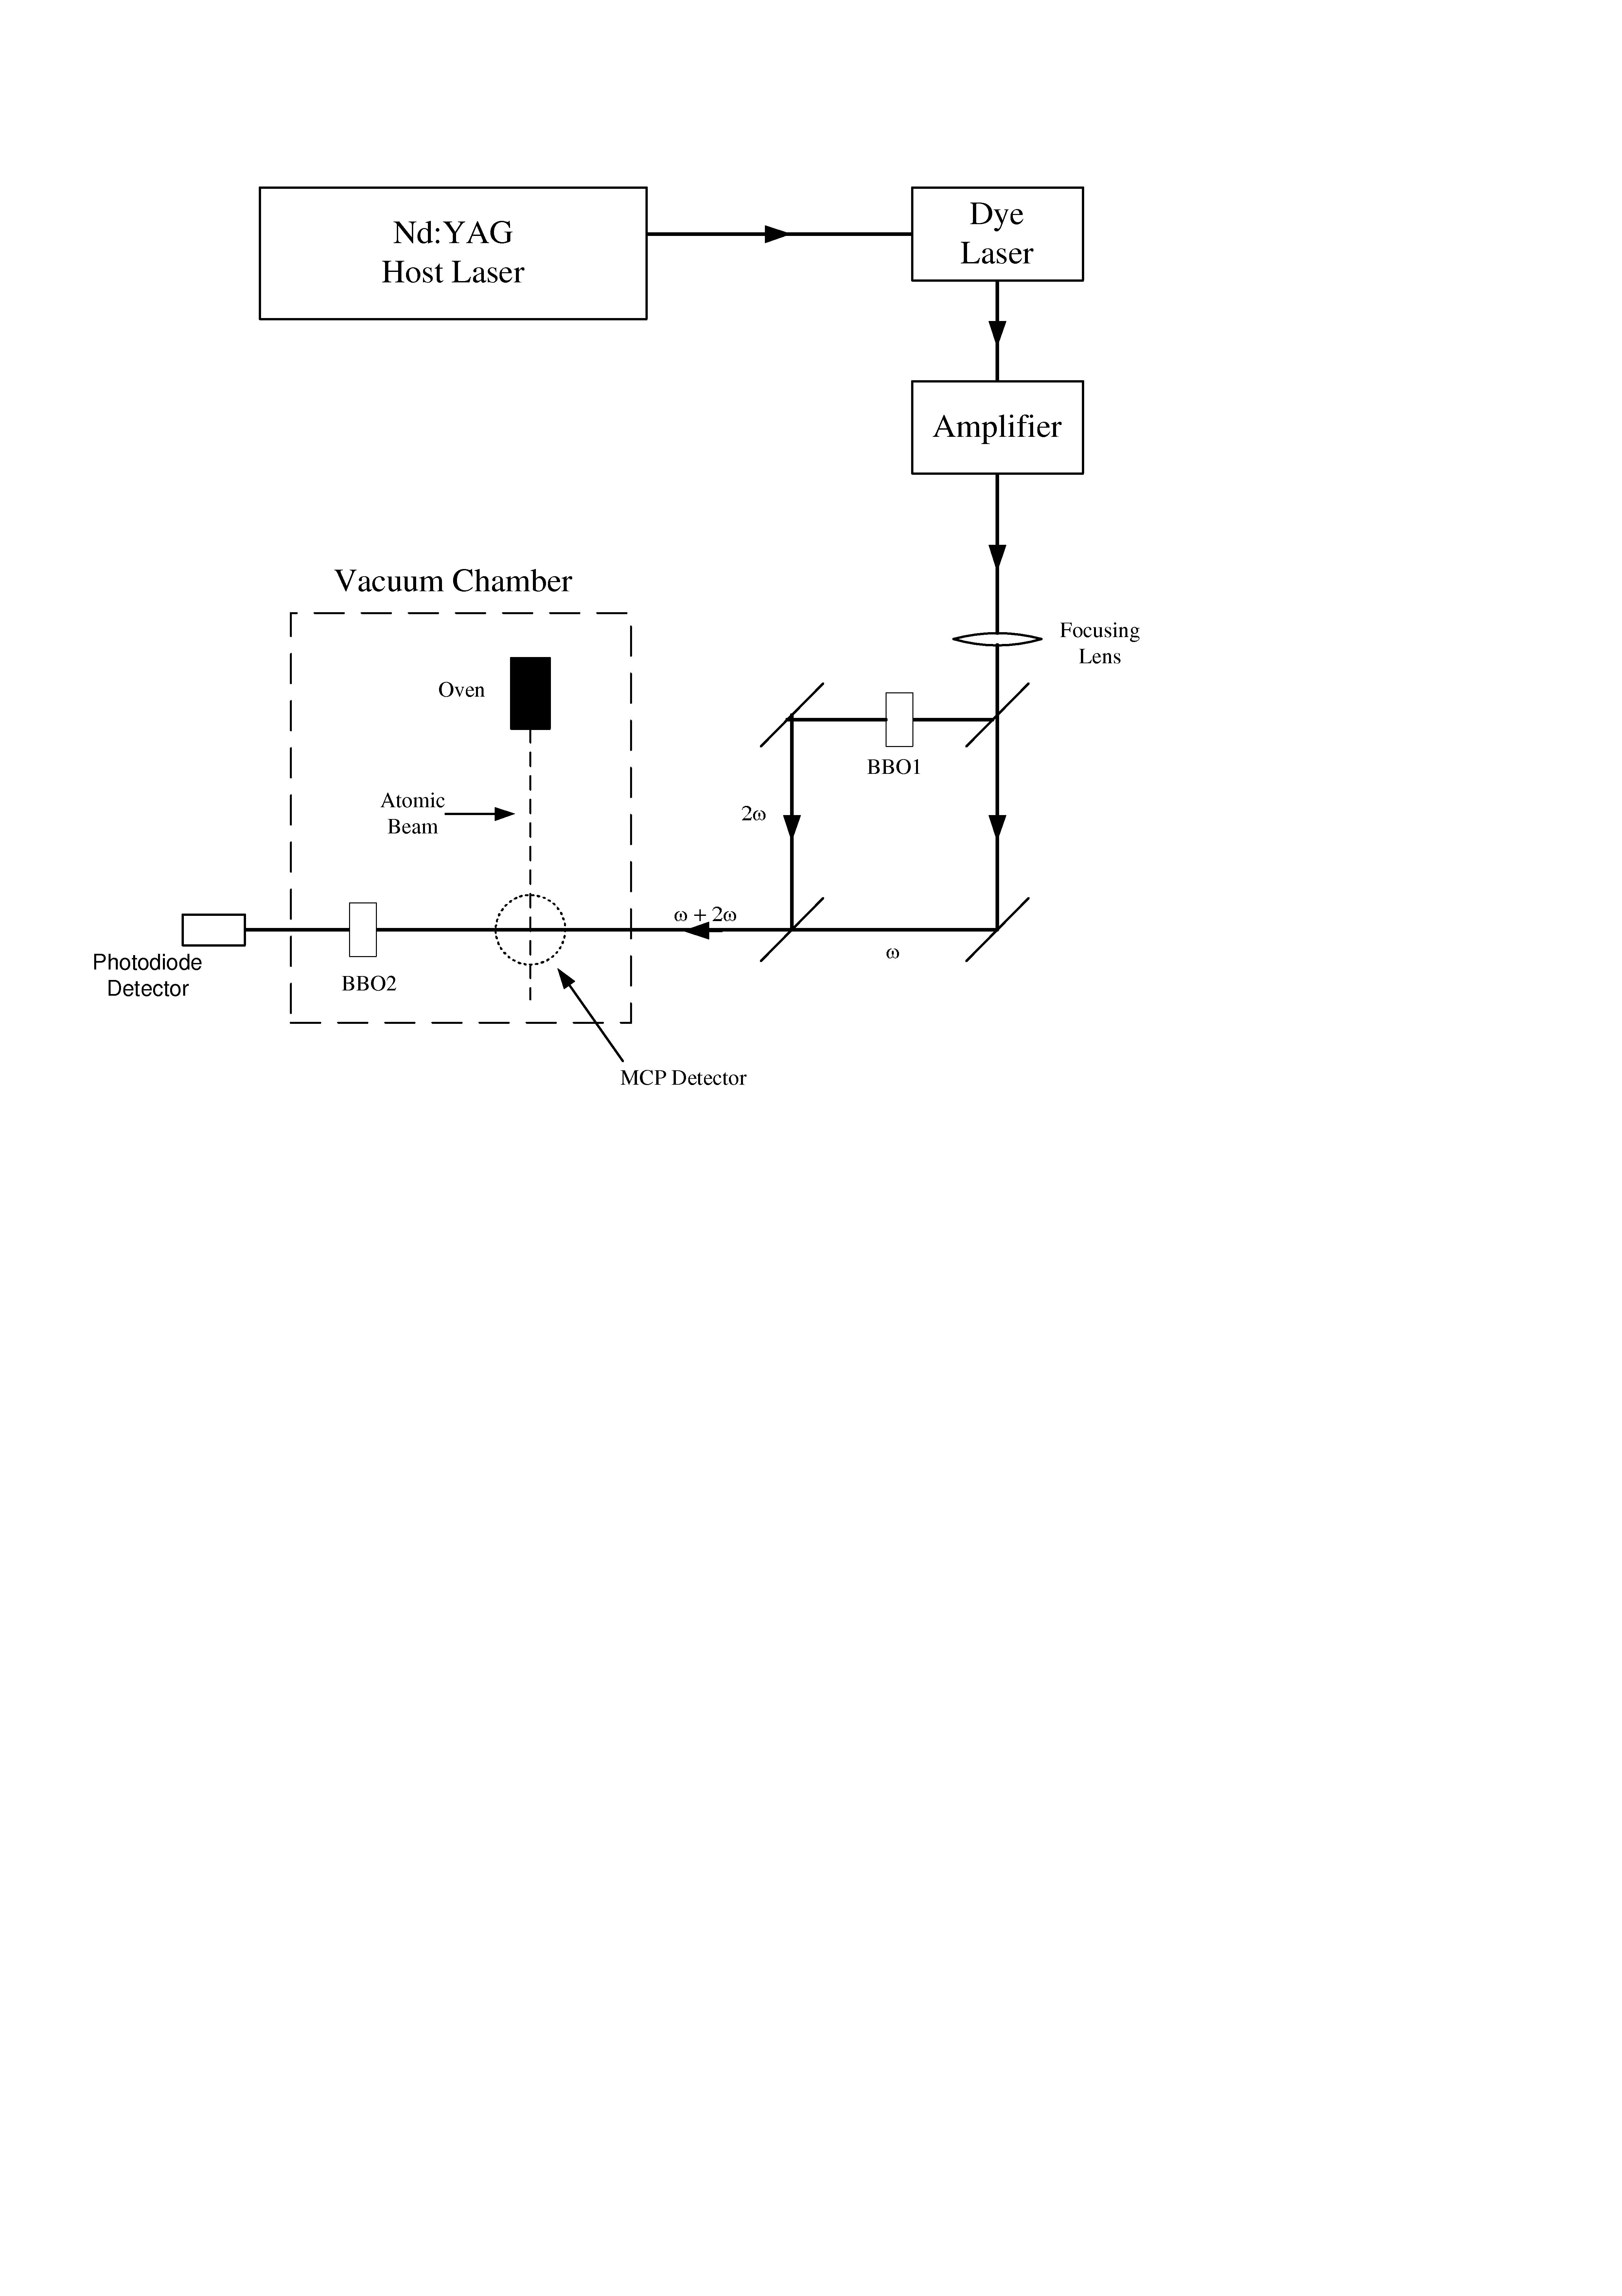
\includegraphics{optsysschem2}
\caption[Experimental setup]{Experimental setup for the
measurement of the phase difference between $p$- and $d$-continuum
waves in atomic rubidium} \label{sysschem}
\end{figure}

A Q-switched Nd:YAG laser is used as a host to excite a tunable
dye laser that produces a pulsed beam at the fundamental frequency
with a wavelength of 560nm.  This will also be known as the
visible beam.  The beam is amplified and passes through a lens
which will focus it close to where the optic/atom interaction will
take place.  Directly after the lens, the beam enters a
Mach-Zehnder-like setup.  In one branch of the setup, the second
harmonic of the fundamental beam is generated using a nonlinear
$\beta$-Barium Borate (BBO) crystal.  The second harmonic beam has
a wavelength of 280 nm and will also be known as the uv beam.  The
two beams are recombined at the output side of the interferometer.
This type setup allows for very good alignment and overlap of the
two beams which is critical for a strong quantum interference
signal to be detected.

Both the visible and uv beams will be focused to a spot inside a
vacuum system close to the point where they will intersect a beam
of rubidium atoms. The point where they intersect is labelled the
interaction region. Located directly above the interaction is the
Micro Channel Plate (MCP) detector which will collect images of
the photoelectron angular distribution.

After travelling from the interaction region, the two beams will
pass through another BBO crystal (BBO2) which will convert some of
the fundamental beam to its second harmonic.  The original second
harmonic beam will pass through the crystal as well and it will
interfere constructively or destructively with the newly generated
second harmonic. The magnitude of the resulting uv beam exiting
the vacuum system is directly related to the relative phase of the
two beams and will be measured using a photodiode.  This is the
essence of the Phase Detector.

\section{Theoretical Photoelectron Angular Distribution}
\label{theopad}

The measurement of the phase difference between the continuum
waves will be accomplished through measurement of photoelectron
angular distribution (PAD) due to a given laser field.  A general
theory for predicting the electron angular distribution of an atom
was developed by Bebb and Gold~\cite{Bebb}.  The experiment was
performed specifically using the ionization of atomic Rubidium by
a two-color field consisting of a frequency and its second
harmonic with crossed linear polarizations.  The theory of Bebb
and Gold was applied specifically to this condition by Wang and
Elliott~\cite{Wang1} and the resulting angular distribution is
shown in equation (\ref{angdist}).


\begin{equation}
\label{angdist} W (\Theta,\Phi) = \frac{m \left| \vec{k}
\right|}{8\pi^2\hbar} \sum_{i,j=\pm} \left| \frac{eE_o^{2\omega}
exp(i\phi^{2\omega})}{2\hbar}O_{ij}^{(1)} +
\frac{e^2(E_o^{\omega})^2
exp(2i\phi^{\omega})}{4\hbar^2}T_{ij}^{(33)}  \right|^2.
\end{equation}

Where $E_o^{\omega}$ and $E_o^{2\omega}$ refer to the electric
field amplitudes of the fundamental field and its second harmonic,
respectively, and $\phi^{\omega}$ and $\phi^{2\omega}$ refer to
the phase of the fundamental and second harmonic fields,
respectively. The applicable spatial components of the one-photon
transition moment, $O_{ij}^{(1)}$, are given by

\begin{eqnarray}
O_{++}^{(1)} &=& \frac{-4\pi i}{\sqrt{6}} e^{i\xi_p} \left[
-Y_{1,1}R_{3/2} + Y_{1,-1} \left(\frac{R_{3/2} + 2R_{1/2}}{3}
\right) \right] \\
O_{--}^{(1)} &=& \frac{-4\pi i}{\sqrt{6}} e^{i\xi_p} \left[
Y_{1,-1}R_{3/2} - Y_{1,1} \left(\frac{R_{3/2} + 2R_{1/2}}{3}
\right) \right] \\
O_{+-}^{(1)} &=& \frac{-4\pi i}{\sqrt{3}} e^{i\xi_p} Y_{1,0}
\left( \frac{R_{3/2} - R_{1/2}}{3} \right) \\
O_{-+}^{(1)} &=& \frac{4\pi i}{\sqrt{3}} e^{i\xi_p} Y_{1,0} \left(
\frac{R_{3/2} - R_{1/2}}{3} \right).
\end{eqnarray}

The spatial components of the two-photon transition moments,
$T_{ij}^{(33)}$, are given by

\begin{eqnarray}
T_{++}^{(33)} &=& \frac{1}{3}e^{i \xi_s}Y_{0,0}S_{\bar{s}} -
\frac{2}{3\sqrt{5}}e^{\xi_d}Y_{2,0}S_{\bar{d}} \\
T_{--}^{(33)} &=& \frac{1}{3}e^{i \xi_s}Y_{0,0}S_{\bar{s}} -
\frac{2}{3\sqrt{5}}e^{\xi_d}Y_{2,0}S_{\bar{d}} \\
T_{+-}^{(33)}&=&
\sqrt{\frac{2}{15}} e^{i\xi_d} Y_{2,1} S_{\Delta d} \\
T_{-+}^{(33)} &=& \sqrt{\frac{2}{15}} e^{i\xi_d} Y_{2,-1}
S_{\Delta d}.
\end{eqnarray}

In the above equations, $Y_{l,m}$ is the spherical harmonic
function, $\xi_{s,p,d}$ is the phase of the $s$, $p$, or $d$
partial wave, and $R_{1/2, 3/2}$ is the single-photon transition
moment. The following substitutions were made.

\begin{equation}
S_{\bar{s}} = \frac{S_1+2S_2}{3} ; S_{\bar{d}} =
\frac{5S_3+S_4+9S_5}{15} ; S_{\Delta d} = \frac{5S_3+S_4-6S_6}{15}
\end{equation}

The terms $S_{1-5}$ refer to the two-photon radial transition
matrix elements.  If the above substitutions are made into
equation (\ref{angdist}), it can be simplified into the following
form.

\begin{eqnarray*}
\label{angdistsimp}
& & W(\Theta,\Phi) \propto\\
& & \left| M_R e^{i\phi_{2 \omega} - 2i\phi_{\omega}}
e^{i(\xi_p-\xi_d)} \frac {-4\pi i}{\sqrt{6}} \left[ -Y_{1,1} +
Y_{1,-1}\frac{1+2 \frac{R_{1/2}}{R_{3/2}}}{3} \right] +
 \left[ \frac{1}{3} e^{i(\xi_s - \xi_d)} Y_{0,0} \frac{S_{\bar{s}}}{S_{\bar{d}}} -\frac{2}{3\sqrt{5}}Y_{2,0} \right] \right|^2  \\
& + & \left|M_R e^{i\phi_{2 \omega} - 2i\phi_{\omega}}
e^{i(\xi_p-\xi_d)} \frac {-4\pi i}{\sqrt{3}} Y_{1,0}\frac{1 -
\frac{R_{1/2}}{R_{3/2}}}{3} +
 \sqrt{\frac{2}{15}} Y_{2,1} \frac{S_{\Delta d}}{S_{\bar{d}}} \right|^2  \\
&  + & \left| M_R e^{i\phi_{2 \omega} - 2i\phi_{\omega}}
e^{i(\xi_p-\xi_d)} \frac {4\pi i}{\sqrt{3}} Y_{1,0} \frac{1 -
\frac{R_{1/2}}{R_{3/2}}}{3} +
 \sqrt{\frac{2}{15}} Y_{2,-1} \frac{S_{\Delta d}}{S_{\bar{d}}} \right|^2 \\
& + & \left| M_R e^{i\phi_{2 \omega} - 2i\phi_{\omega}}
e^{i(\xi_p-\xi_d)} \frac {-4\pi i}{\sqrt{6}} \left[ Y_{1,-1} -
Y_{1,1}\frac{1+2 \frac{R_{1/2}}{R_{3/2}}}{3} \right] +
 \left[ \frac{1}{3} e^{i(\xi_s - \xi_d)} Y_{0,0} \frac{S_{\bar{s}}}{S_{\bar{d}}} -\frac{2}{3\sqrt{5}}Y_{2,0} \right]
 \right|^2,
\end{eqnarray*}where $M_R$ is the relative magnitude of the one-photon process to
that of the two-photon process.  It can clearly be seen from
equation (\ref{angdistsimp}) that in order to determine the
continuum phase difference, $\xi_p-\xi_d$, from a fit to this
equation, it is necessary to know the optical phase difference,
$\phi_{2 \omega} - 2\phi_{\omega}$.
 Many of the quantities of equation (\ref{angdistsimp}) have been
previously determined by Wang and Elliott~\cite{Wang1, Wang2}.
These quantities are shown in table (\ref{angdistvalues}).

\begin{table}[h]
\caption[Known Quantities in Angular Distribution Function]{Values
of known quantities used in equation (\ref{angdistsimp})}
\label{angdistvalues}
  \centering
\begin{tabular}{|c|r|}
\hline
Quantity&Value\\
\hline
$\frac{R_{1/2}}{R_{3/2}}$&1.96\\
$\frac{S_{\bar{s}}}{S_{\bar{d}}}$&-0.42\\
$\frac{S_{\Delta d}}{S_{\bar{d}}}$&-0.36\\
$\xi_s-\xi_d$&2.08\\
\hline
\end{tabular}

\end{table}

Using equation (\ref{angdistsimp}) and the properties of the
detector system used by Wang~\cite{Wang0} it is possible to
develop expected angular distributions and the corresponding
images that will be detected.  Some example calculated images are
shown in figure (\ref{extheo}).

\begin{figure}
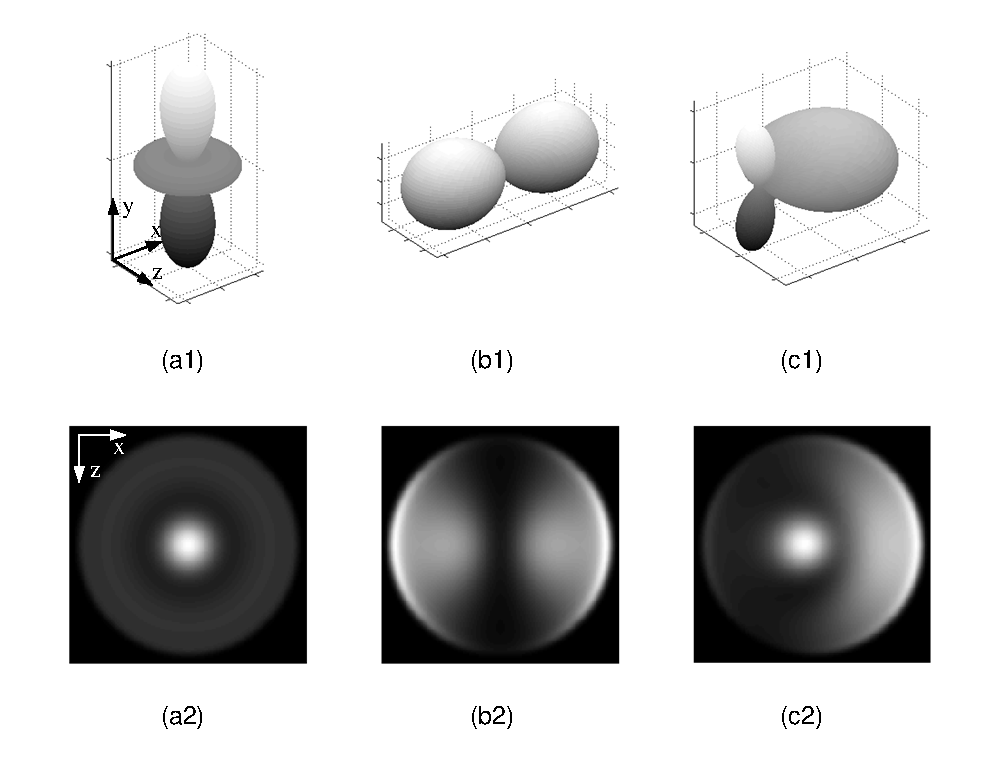
\includegraphics{extheo}
\caption[Example theoretical angular distributions and
images]{Examples of various angular distributions, (x1), and their
corresponding images, (x2) on the detector system.  Images (a1,2)
represent the result of excitation due to a field of wavelength
560 nm that is vertically polarized.  Images (b1,2) are due to a
horizontally polarized field at 280 nm.  Images (c1,2) represent a
result having both fields present.} \label{extheo}
\end{figure}
   %Introduction

\chapter{Theory}

Uniquely determining the phase difference between the $p$- and
$d$- continuum waves requires knowledge of the relative optical
phase of the two optical fields present at the interaction.  The
goal is to determine the optical phase difference, $\phi_{2
\omega} - 2\phi_{\omega}$, between the fundamental field and its
second harmonic at the interaction region.  This can be done by
using a second non-linear crystal to generate a co-linear second
harmonic beam and then looking at the magnitude of the
interference signal between the two second harmonic
beams~\cite{Chudinov}. The method makes use of the fact that,
during second harmonic generation, the harmonic field has a
definite phase relationship to that of the fundamental.  In our
experiment, both beams leave the interaction region and travel
some distance, $d$, inside the vacuum system. They then pass
through a BBO crystal where some of the visible beam is converted
into its second harmonic. At the output of the BBO crystal there
are now two second harmonic fields that will interfere
constructively or destructively depending on their relative phase.
The amplitude of the interfering beams will go as the square of
the cosine of the phase difference between them.  Therefore, by
measuring the amplitude of the interference signal, the relative
phase between the visible and uv fields at the interaction region
can be determined.

Careful consideration must be made with respect to two things when
using this method.  The first is that, as these two focused
Gaussian beams travel from their focus into the far-field, a phase
difference will develop between them.  The second is that there
will be some phase difference between the visible beam and the
second harmonic that is created from it within the BBO.  If these
are both accounted for, the optical phase difference at the
interaction region can eventually be determined correctly.


\section{Clarification of Coordinate Systems}

In performing this experiment, it is necessary to define and
adhere to a coordinate system in order to avoid confusion.  In
most cases, it is convenient to define the coordinates with
respect to the travelling optical beam.  For these cases, a
coordinate system is defined in the following way. The positive
$z$-axis points in the direction of the beam's propagation. The
positive $y$-axis is normal to or up from the optical table, and
the $x$-axis is located accordingly to create a right-handed
coordinate system.

When dealing with crystal structures, it is often more convenient
to define a coordinate system that coincides with the particular
axes of the crystal.  The type of crystal that is under study is a
uniaxial crystal, which means that light polarized along one axis
experiences a different index of refraction than does light
polarized along the other two.  This axis will be designated the
optic axis and light polarized along it will be said to be
experiencing an extraordinary refractive index. Light polarized
along either of the other two axes will be experiencing an
ordinary refractive index. In a crystal, it is customary to
designate the optic axis as the $Z$-axis, which means that the
$X$- and $Y$-axes will be used to designate the ordinary axes. For
our purposes, the $X$- and $Y$-axes will be interchangeable.

The convention used here is to designate the laboratory
coordinates in lower case ($x,y,z$) and the crystal coordinates in
upper case ($X,Y,Z$).  A diagram of these coordinates is shown in
figure(\ref{coord}).

\begin{figure}
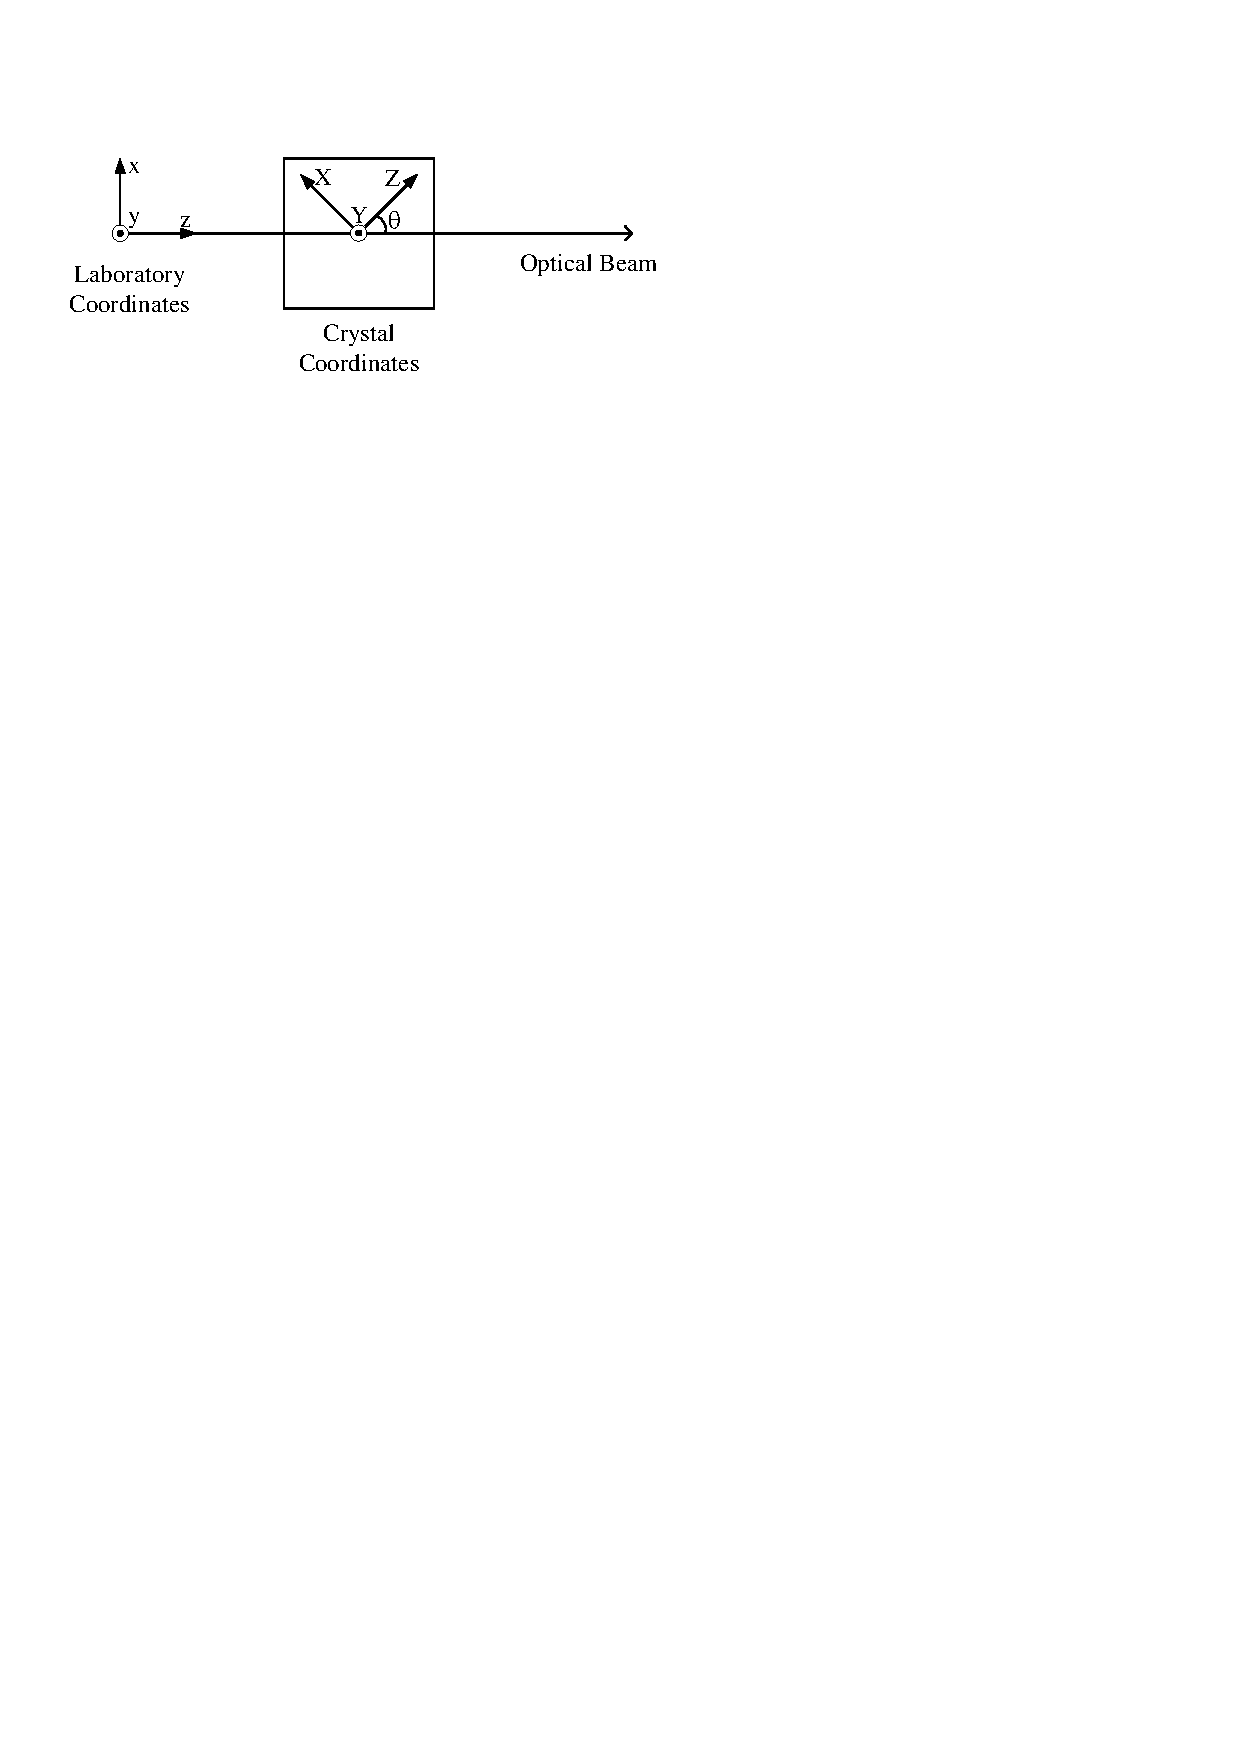
\includegraphics{coordsys2}
\caption[Definition of coordinate systems used]{Diagram showing
the two types of coordinate systems used.  Coordinates in lower
case are defined with respect to the laboratory environment and
coordinates in upper case are defined with respect to the
crystalline axes.}
\label{coord}%
\end{figure}


\section{Shift During Propagation}
\label{phaseshiftff}

We can consider the visible and uv beams to be focused Gaussian
beams.  In our reference frame, these beams are travelling in the
$+z$ direction and the beams are focused at the point $z=0$. The
focal point is placed before the interaction region at the point
$z=z_i$ for reasons discussed below.  The second BBO doubling
crystal is located some distance, $d$, after the interaction
region.  Refer to figure (\ref{opdcalc}) for an illustration of
terms used.

\begin{figure}
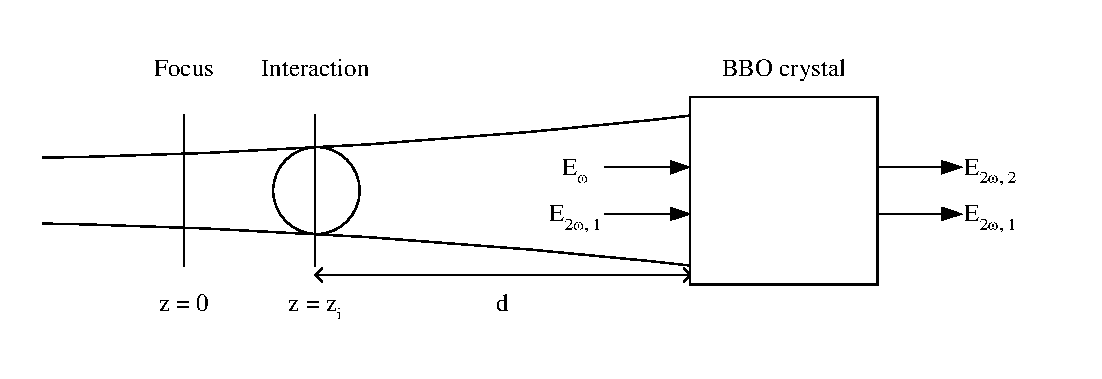
\includegraphics{focusshift}
\caption[Method for determining interaction optical phase
Difference]{Illustration of the method used to determine the
Optical Phase Difference at the interaction region}
\label{opdcalc}
\end{figure}


If we assume an electric field of the form $E(z)=E_oe^{i\phi(z)}$
then, for a Gaussian beam, the phase changes with propagation
according to~\cite{Verdeyen}

\begin{equation}\label{phiz}
\phi(z)=-kz+\arctan{\left[\frac{z}{z_o}\right]},
\end{equation} where $k$ is the wave vector of the beam, and $z_o$ is the beam's
confocal parameter. It should be noted that a second harmonic beam
will have both the same focal point and the same value of $z_o$ as
the fundamental wave from which it was created~\cite{Kleinman}.

We are ultimately interested in determining the value of the
optical phase difference at the interaction region,
$\Delta\phi_{i}=\phi_{2\omega}-2\phi_\omega$.  We can say that the
change in phase between the two fields as they travel the distance
to the BBO equals the change in phase of the visible beam minus
the change in phase of the uv beam.

\begin{equation}\label{opd1}
\Delta\phi_d-\Delta\phi_{i}=\Delta\phi_{2\omega}-2\Delta\phi_\omega
\end{equation}

In the above equation, $\Delta\phi_{2\omega}$ and
$\Delta\phi_\omega$ can be determined by using the fact that these
are focused Gaussian beams and they obey equation (\ref{phiz}).
Phase difference during propagation due to dispersion can be
ignored since the two beams are travelling in a high vacuum
environment which can be considered effectively free from
dispersion.

Knowing this, $\Delta\phi_{2\omega}$ in equation (\ref{opd1}) can
be found.

\begin{eqnarray}
\Delta\phi_{2\omega}& & = \left. \phi_{2\omega} \right|_{z=z_i+d} - \left. \phi_{2\omega} \right|_{z=z_i} \\
& & = \left[ -k_{2\omega}(z_i+d)+\arctan{\frac{z_i+d}{z_o}}
\right] - \left[ -k_{2\omega}z_i+\arctan{\frac{z_i}{z_o}} \right]
\label{opd2}
\end{eqnarray}

Similarly,

\begin{equation}\label{opd3}
\Delta\phi_\omega = \left[
-k_{\omega}(z_i+d)+\arctan{\frac{z_i+d}{z_o}} \right] - \left[
-k_{\omega}(z_i)+\arctan{\frac{z_i}{z_o}} \right].
\end{equation}

Since the uv beam has double the frequency of the visible beam,
the wave vectors of the two beams are related by:
$k_{2\omega}=2k_\omega$.  Accounting for this and substituting
equations (\ref{opd2}) and (\ref{opd3}) into equation (\ref{opd1})
yields

\begin{equation}\label{opd4}
\Delta\phi_{d}-\Delta\phi_{i}=-\arctan{\frac{z_i+d}{z_o}}+\arctan{\frac{z_i}{z_o}}.
\end{equation}

As $d$ becomes large relative to $z_o$, the the first term of
equation (\ref{opd4}) approaches $-\frac{\pi}{2}$.  In our
experimental setup, $z_o$ is on the order of a few millimeters and
$d$ is about 40 cm and so the first term will be taken as
$-\frac{\pi}{2}$.

If we look at the second term of equation (\ref{opd4}), we can see
the reason for placing the focus slightly before the interaction
region.  The arc tangent function is rapidly varying when its
argument approaches zero, therefore, choosing a value of $z_i$
that is very small could potentially introduce a large amount of
error in the final calculation of the phase difference.  If $z_i$
is chosen to be a bit larger, small errors in the location of the
focus will have less of an overall impact on the phase
measurement.  In the end, the phase difference will have to be
adjusted by this factor.


\section{Shift during Second Harmonic Generation}

In second harmonic generation (SHG), the newly generated field
will have a definite phase relationship to that of its driving
field. In general, this phase difference is non-zero and so it
must be determined in order for us to determine the phase
relationship between the visible and uv beams at the interaction.
To calculate this, we must look at the second harmonic generation
process.

In our experiment, a second harmonic field is generated using the
nonlinear crystal $\beta$-Barium Borate or BBO.  It is classified
as a negative uniaxial crystal and it has a crystal class of 3$m$.
The crystal used was cut for Type I SHG at a phase matching angle
that corresponds to the fundamental wavelength of 560nm. In Type I
SHG, the fundamental and second harmonic fields are linearly
polarized and perpendicular to each other.  The phase matching
angle, $\theta$, is the angle between the optic axis of the
crystal and the propagation direction of the optical beam at which
both the fundamental and second harmonic beams have the same phase
velocity within the crystal.  In BBO, this angle is $44.4^\circ$
for a fundamental wavelength of 560nm.

\subsection{Nonlinear Optics Background}
\label{NLO}%

The nonlinear effects arise from the fact that the material
exhibits a non-linear susceptibility.  In general, the
polarization of a material, $P$, may be described by

\begin{equation}\label{pol}
P=\epsilon_o \chi E,
\end{equation} where $\chi$ is known as the susceptibility of the material, which
may be non-linear.  Expanding equation (\ref{pol}) for the case of
a non-linear susceptibility yields

\begin{equation}\label{polexpansion}
\begin{array}{cccccccc}
P&=&P^{(1)}&+&P^{(2)}&+&P^{(3)}&+ ...\\
&=&\epsilon_o\chi^{(1)}E&+& \epsilon_o\chi^{(2)}E^2&+& \epsilon_o\chi^{(3)}E^3&+ ... \\
\end{array}
\end{equation}

We will be primarily concerned with the second order
susceptibility, $\chi^{(2)}$, since it contributes to second
harmonic generation and it offers a far greater contribution than
do all other higher order terms.  In general, $\chi^{(2)}$ is a
second order tensor.  Under certain symmetry conditions and using
the relation $d_{ijk}=\frac{1}{2}\chi^{(2)}_{ijk}$, equation
(\ref{polexpansion}) can be written in the following condensed
form which accounts for all possible orientations.~\cite{RWBoyd}


\begin{equation}\label{darray}
\left[ \begin{array}{c} P_X \\
P_Y \\
P_Z \end{array} \right]= 2 \left[ \begin{array}{cccccc}
d_{11} & d_{12} & d_{13} & d_{14} & d_{15} & d_{16} \\
d_{21} & d_{22} & d_{23} & d_{24} & d_{25} & d_{26} \\
d_{31} & d_{32} & d_{33} & d_{34} & d_{35} & d_{36} \\
\end{array}\right]
\left[ \begin{array}{c} E_X^2 \\
E_Y^2 \\
E_Z^2 \\
2 E_Y E_Z \\
2 E_X E_Z \\
2 E_X E_Y \\
\end{array} \right],
\end{equation} where $E_i$ is the magnitude of the electric field polarized in
the $i$ direction.  For a fixed polarization and propagation
direction, equation (\ref{darray}) may be further abbreviated to
the form

\begin{equation}\label{P2dE}
P^{(2)}(z,t)=2 d_{eff}E^2(z,t).
\end{equation}

If we assume an electric field of form, $\label{efield} E(z,t) =
\frac{1}{2} \left[ Ee^{i(\omega t-kz)} + c.c.\right]$, and take
the square of it, equation(\ref{P2dE}) becomes

\begin{equation}\label{pol2}
P^{(2)}=2 d_{eff} \left[ Ee^{2i(\omega t-kz)} + c.c. + 2\left| E
\right|^2 \right].
\end{equation}

This nonlinear polarization consists of two parts.  One part, $2
d_{eff} \left[ Ee^{2i(\omega t-kz)} + c.c. \right]$, consists of a
field oscillating at twice the original frequency which is
responsible for second harmonic generation.  The other part, $2
d_{eff} \left[ 2\left| E \right|^2 \right]$, contributes to what
is known as optical rectification.  It can be seen that this is a
polarization that does not vary with time.

\subsection{Second Harmonic Generation Process}
\label{SHG}

We now want to relate the electric field of the fundamental beam
entering the crystal to the second harmonic that is generated.
This can be done through use of Maxwell's equations and the wave
equation.

\begin{equation}\label{waveeqn}
-\nabla^2 E + \frac{1}{c^2} \frac{\partial^2}{\partial t^2} E =
\frac{-4\pi}{c^2} \frac{\partial^2 P}{\partial t^2}
\end{equation}


By using an electric field of the form $\label{efield}
E_{\omega}(z,t) = \frac{1}{2} \left[ Ee^{i(\omega t-kz)} + c.c.
\right]$ and equation(\ref{P2dE}),  and by making the
approximations of perfect phase matching and an undepleted
fundamental beam, equation(\ref{waveeqn}) reduces to~\cite{Yariv}

\begin{equation}\label{shgeqn}
E_{2\omega}= -i \omega \sqrt{\frac{\mu_o}{\epsilon}} d_{eff}
E_{\omega} E_{\omega} L.
\end{equation}

In the above equation, $\omega$ is the fundamental frequency,
$\mu_o$ is the magnetic susceptibility of free space, $\epsilon$
is electric permeability of the crystal, and $L$ is the length of
the crystal. The amplitudes of the second harmonic and fundamental
fields are given by $E_{2\omega}$ and $E_{\omega}$, respectively.
Also, $d_{eff}$ is defined as half of the second order nonlinear
susceptibility. According to Eimerl~\cite{Eimerl}, in crystal of
class 3$m$, $d_{eff}$ can be found by

\begin{equation}\label{deff}
d_{eff}=d_{31}\sin{\theta} - d_{22}\cos{\theta}\sin{3\phi},
\end{equation} where $\theta$ is the angle between the beam's wave vector and the
crystalline $Z$-axis and $\phi$ is the angle between the wave
vector and the crystal's $X$-$Z$ plane.  The crystal used for this
experiment is cut, for a beam with normal incidence to the
surface, with angles of $\theta=44.4^\circ$ and $\phi=0^\circ$.

From equation (\ref{shgeqn}), it can be seen that the phase of the
second harmonic field differs from that of the fundamental due to
the \(-i\) factor in equation (\ref{shgeqn}). This phase may also
be affected by the sign on \(d_{eff}\) which may be either
positive or negative, and depends on the relative orientation
between the crystal's optic axis and beam direction. Overall, this
correlates to a phase shift during SHG of either $-\frac{\pi}{2}$
or $+\frac{\pi}{2}$.  Combining this with the result of section
(\ref{phaseshiftff}) yields an overall phase shift from the beam's
focus to the phase detector of either $0$ or $\pi$.  In order to
resolve this ambiguity, we must determine the sign of $d_{eff}$.

It can be seen in equation (\ref{pol2}) that the term $d_{eff}$ is
common to both the second harmonic generation and the optical
rectification processes.  Therefore, if the sign of $d_{eff}$ can
be determined by measuring the optical rectification, then it will
also be known for the second harmonic generation process.

In summary, if we combine the results of sections
(\ref{phaseshiftff}) and (\ref{SHG}) we can arrive at an
expression for the total phase shift, $\Delta\phi_{total}$, that
occurs between the fundamental and second harmonic in travelling
from the interaction to the phase detector.

\begin{equation}
\begin{array}{cccccc}
\Delta\phi_{total}&=&-\arctan{\frac{z_i+d}{z_o}}&+&\angle \left[-i \cdot \mbox{sign}(d_{eff}) \right] &\\
                  &\approx& -\frac{\pi}{2}       &+&\angle \left[-i \cdot \mbox{sign}(d_{eff})  \right]&\mbox{for}\ z_i+d\gg z_o\\
                  &=& \left\{ \begin{array}{cccccc}
                  -\frac{\pi}{2}&+& -\frac{\pi}{2}&=&\pi &\mbox{for}\ d_{eff} >  0 \\
                  -\frac{\pi}{2}&+& \frac{\pi}{2}&=&0 &\mbox{for}\ d_{eff} < 0
                  \end{array} \right.
\end{array}
\end{equation}

\subsection{Optical Rectification}

Optical rectification is the process of generating a DC electric
field from a time-varying optical field.  An expression for the
polarization that arises from an optical rectification process was
derived in section (\ref{NLO}).

\begin{equation}\label{ORpol}
P_{DC}^{(2)}=2d_{eff} \left| E\right|^2.
\end{equation}

In our experiment, linearly polarized light is used in a Type I
phase matching configuration and this generates both a second
harmonic signal and an optical rectification signal.  The two
generated fields will have polarization perpendicular to that of
the input field. Let us assume that the input field is polarized
in the $y$-direction and that it is intersecting the crystal's
optic axis and some angle, $\theta$.  The exact orientation of the
crystal axes is not known, so an orientation is assumed for the
purposes of this derivation.  The angle that the wave vector makes
with the crystal's optic axis is known, however, due to the phase
matching condition for generation of second harmonic.  The
relative orientations of the crystalline axes and the laboratory
coordinates are shown in figure (\ref{crysorient}).

\begin{figure}
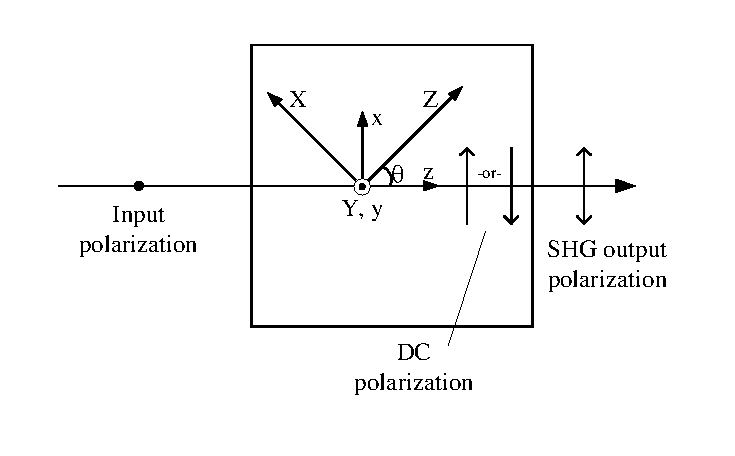
\includegraphics{polcryst}
\caption[Relative orientation of crystal and laboratory coordinate
systems]{Diagram of the relative orientations of the crystal and
laboratory coordinate systems}
\label{crysorient}%
\end{figure}

Since the beam is propagating in the $z$-direction, we can arrive
at an expression for the resulting DC polarization, written in the
laboratory coordinate system.  In order to obtain this expression,
we begin with the equation relating polarization to electric field
that was given in equation (\ref{darray}).  For a specific crystal
class, certain symmetry conditions may restrict certain values in
the $d_{ij}$ matrix to be zero or equal to other values in the
matrix. Since we are considering specifically a BBO crystal we may
use the reduced form for crystals of class 3$m$, of which BBO is a
member~\cite{RWBoyd}.

\begin{equation}\label{BBOdarray}
\left[ \begin{array}{c} P_X \\
P_Y \\
P_Z \end{array} \right]= 2 \left[ \begin{array}{cccccc}
0 & 0 & 0 & 0 & d_{15} & -d_{22} \\
-d_{22} & d_{22} & 0 & d_{15} & 0 & 0 \\
d_{31} & d_{31} & d_{33} & 0 & 0 & 0 \\
\end{array}\right]
\left[ \begin{array}{c} E_X^2 \\
E_Y^2 \\
E_Z^2 \\
2 E_Y E_Z \\
2 E_X E_Z \\
2 E_X E_Y \\
\end{array} \right].
\end{equation}

Note that the indices are given in terms of the crystal coordinate
axes.  Since the input field consists only of an electric field
linearly polarized in the $Y$-direction, equation
(\ref{BBOdarray}) reduces to

\begin{equation}
\label{crystalpol}
\begin{array}{ccc}
P_Y &=& 2d_{22}E_Y^2 \\%
P_Z &=& 2d_{31}E_Y^2. \end{array}.
\end{equation}

From this, we are interested only in the component of the
polarization that is in the $x$-direction in our laboratory
coordinate system.  In other words, we want the component that is
orthogonal to the input field and the propagation direction, which
is the result of a Type I process.  Transforming equation
(\ref{crystalpol}) into the laboratory coordinate system, the
polarization in the $x$-direction is given by

\begin{equation}
P_x=2d_{31} \sin{\theta} E_y^2,
\end{equation} and the DC polarization corresponding to this is

\begin{equation} \label{ORpolsign}
P_x=2d_{31} \sin{\theta} \left| E_y\right|^2 .
\end{equation}


This result can be verified by comparing to equation (\ref{P2dE})
and recognizing that $d_{eff}=d_{31} \sin{\theta}$ for $\phi=0$
from equation(\ref{deff}).  Since we do not know the actual
orientation of the crystal's positive $Z$-axis, we can say that we
do not know the sign of $\sin{\theta}$, and we therefore do not
know the sign of $d_{eff}$.  The problem of finding the sign of
$d_{eff}$ now comes to determining the direction of the DC
polarization that is developed in the crystal.

In order to measure this DC polarization, conducting electrodes
are placed on the sides of the crystal perpendicular to the
expected DC polarization vector.  The polarization will be
developed within the area of the laser beam in the crystal.  This
polarization corresponds to some density of dipoles, all oriented
in the same direction.  Within the crystal, this will appear as a
separation of charge with one edge of the laser beam appearing to
have a positive charge and the other appearing to have a negative
charge.  These charges will induce opposite charges on the
conducting electrodes, and thus there will be a voltage difference
between the two electrodes which can be measured.  An illustration
of this is shown in figure (\ref{polcharge}).

\begin{figure}
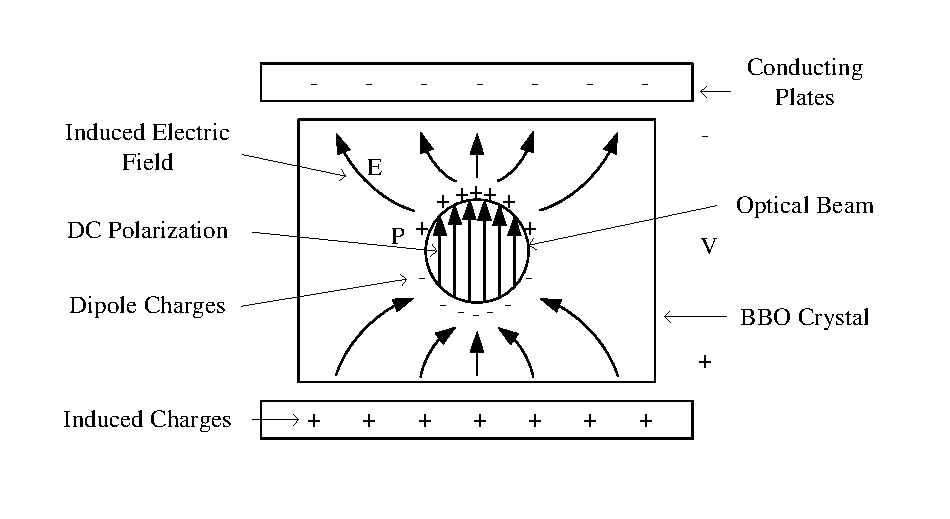
\includegraphics{polcharge}
\caption[Effect of DC polarization in BBO crystal]{Method used to
detect the polarization direction.  The DC polarization causes a
separation of charge within the crystal which, in turn, induces
charges on the conducting plates.  The difference in charge on the
plates corresponds to a voltage and the direction of the voltage
drop can be used to find the polarization direction.}
\label{polcharge}%
\end{figure}

There are two possible cases that may arise, corresponding to
possible signs of $d_{eff}$. Either the measured voltage will
correspond to a DC field which points in the positive
$x$-direction or in the negative $x$-direction. It can be seen
from equation (\ref{ORpolsign}) that a positive value of $d_{eff}$
will yield a polarization in the positive $x$-direction and a
negative value of $d_{eff}$ will yield a polarization in the
negative $x$-direction. An illustration of these two cases is
shown in figure (\ref{ORresult}).


\begin{figure}
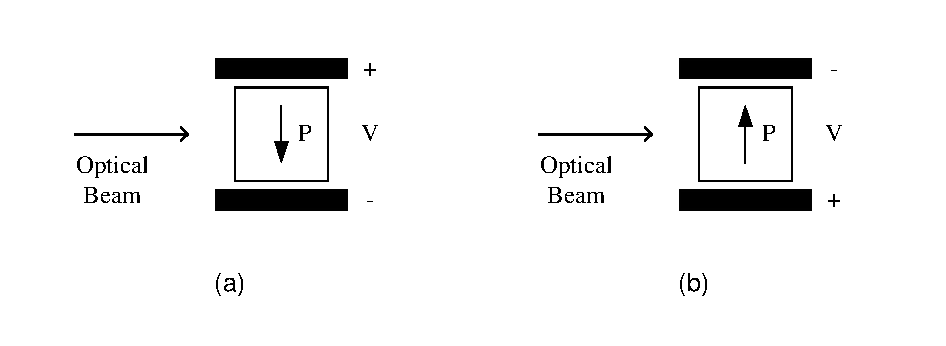
\includegraphics{ORresult}
\caption[Possible results of optical rectification
measurement]{Diagram showing the two possible results of an
optical rectification measurement, including the resulting induced
voltage.}
\label{ORresult}%
\end{figure}
  %Theory

\chapter{Experiment and Results}

\section{Measurement of Optical Rectification}

We are interested simply in measuring the sign of $d_{eff}$ and
this can be done by measuring the direction of the DC electric
field that is generated within the crystal.  Since optical
rectification is a second order process, a rather large electric
field must be used in order to see some result; it must be
comparable to that used to generate second harmonic fields.  In
our current setup we employ a Q-switched Nd:YAG laser capable of
producing pulses with energies of up to 100 mJ of 10 ns duration
at a wavelength of 532 nm. If we approximate the pulse as a square
pulse in time, then this correlates to a peak power of 10 MW.

The DC electric field is measured by placing parallel conducting
plates perpendicular to the field and then measuring the voltage
that is induced across them.  A diagram of the configuration used
to make this measurement is shown in figure (\ref{ORexp}).

\begin{figure}
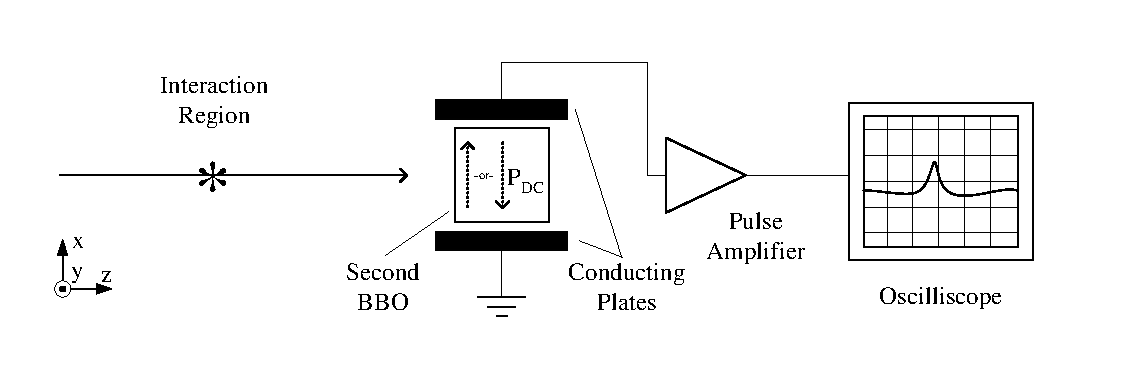
\includegraphics{ORexp}
\caption[Optical rectification measurement apparatus]{Diagram of
the experimental setup used to measure the optical rectification
signal in a BBO crystal}
\label{ORexp}%
\end{figure}

The crystal used in this experiment is a $\beta$-Barium Borate
(BBO) that has an open face of 5mm$\times$4mm and is 5mm in
length. It is oriented for Type I phase matching which means that
the fundamental field and the harmonic field are polarized
perpendicularly to one another.  In this case, the fundamental
field has a polarization along one of the crystal's ordinary axis,
and the second harmonic, as well as the optical rectification
signal, are created along the extraordinary axis. These
orientations are also shown in figure (\ref{ORexp}).

While the short duration pulses from the Nd:YAG laser do allow for
higher peak power, they also make the DC measurement more
difficult since the DC field is essentially only present when the
optical field is driving it.  We therefore need a fast detector
that is capable of detecting the polarity of pulses of 10 ns
duration.

[amplifier/scope configuration]

\section{Choice of Laboratory Coordinate System}

Care must be taken in adhering the laboratory coordinate system.
Since our goal is only to determine the sign of the term
$d_{eff}$, any error in the orientation of the coordinates may
have the result of changing the result to its opposite.  All
calculations and measurements must adhere to these coordinates for
the same reason. These include the phase shift in moving to the
far field, the orientation of the camera imaging system, the
experimental image fitting program, and the orientation of the
phase detection BBO.

Recall, that the coordinate system is defined in the following
way. The positive $z$-axis points in the direction of the beam's
propagation, and the positive $y$-axis is normal to the optical
table.

The first thing that must be accounted for is the orientation of
the camera in the imaging system.  The camera is positioned
looking down on the interaction region, with the optical beam
entering from the top of the image.  Therefore, the collected
image lies in the $x$-$z$ plane with the origin in the upper left corner of the image.  

%positive directions as indicated in figure (\ref{imgcoord}).

%\begin{figure}
%\includegraphics{imgcoord}
%\caption[Image coordinates]{Example experimental image showing the
%orientation of the coordinate system}
%\label{imgcoord}%
%\end{figure}

This experiment uses an algorithm to fit the theoretical equations
to the experimental images.  Since the expected images will be
asymmetric, it is important that the coordinate system used in the
program coincides with that of the image that is passed to it.
Therefore, care must be taken to insure that the orientations of
the spherical harmonics in equation (\ref{angdistsimp}) match
correctly.

Finally, the sign of $d_{eff}$ that is measured will depend on the
choice of coordinate system as well.  Since we are using Type I
phase matching in the second doubling crystal and the incoming
electric field polarization is vertical (in the $z$ direction) we
expect the polarization of the second harmonic as well as the
optical rectification field to be horizontal (in the $x$
direction).  Therefore, we expect

\begin{equation}
P^{(2)}_x = 2d_{eff} \left| E_y \right|^2.
\end{equation}

Determining the sign of $d_{eff}$ now comes to determining if the
DC polarization points in the positive or negative $x$-direction
in our coordinate system.

\section{Determination of Optical Rectification Direction and Optical Phase Shift}





\section{Verification of Independence of Choice of Coordinate System}

Since it appears that the determination of the phase shift depends 
only on the choice of coordinates, some confusion may arise from 
the seemingly abitrary choice of coordinate system.  It appears that
if we measure a polarization in one direction and then choose the
positive $x$-direction to coincide with that, we will end up with a 
$-\frac{\pi}{2}$ phase shift during SHG.  If we were to choose the 
positive $x$-direction to be opposite, then we will end up with a 
$-\frac{\pi}{2}$ phase shift.  The confusion stems from the fact that 
we are trying to determine the phase difference between two waves that
are polarized in planes perpendicular to each other.

Let us consider an example of two waves of the same frequency polarized 
perpendicularly to each other.  This situation is illustrated in figure
(\ref{perppol}).  The reference wave will be the one polarized perpendicularly
to the plane of the page and the positive direction will be up from the
plane of the page.  If we choose the $a$-direction to be positive, then the
two waves will have zero phase difference.  However, if we choose the $a'$-direction
to be positive, then the two waves will have a phase difference of $\pi$.
Since the calculated phase shift during SHG is not the only thing that 
changes with a change in coordinate system we can begin to see that 
if we choose and adhere to a coordinate system properly, confusion in 
the phase can be eliminated.

\begin{figure}
%\includegraphics{}
\caption[Relative phase of perpendicularly polarized waves]{Relative 
phase of perpendicularly polarized waves}
\label{perppol}
\end{figure}


In the end, it must be true that our determination of the phase
shift that occurs during second harmonic generation must be
independent of our choice of coordinate systems.  The result
should stay the same for any choice.  In order to verify this we
will select an alternate coordinate system, and demonstrate that
the final result remains unchanged.  We must therefore track all
points where the change in coordinates will affect the calculated phase of
the beams.

We will start with a single configuration in our current
coordinate system, and then repeat with a different coordinate
system. The physical aspects of each configuration will remain the
same, that is, the collected image and the direction of the
optical rectification signal will not change.  The two situations
are illustrated in figure (\ref{inde}).

\begin{figure}
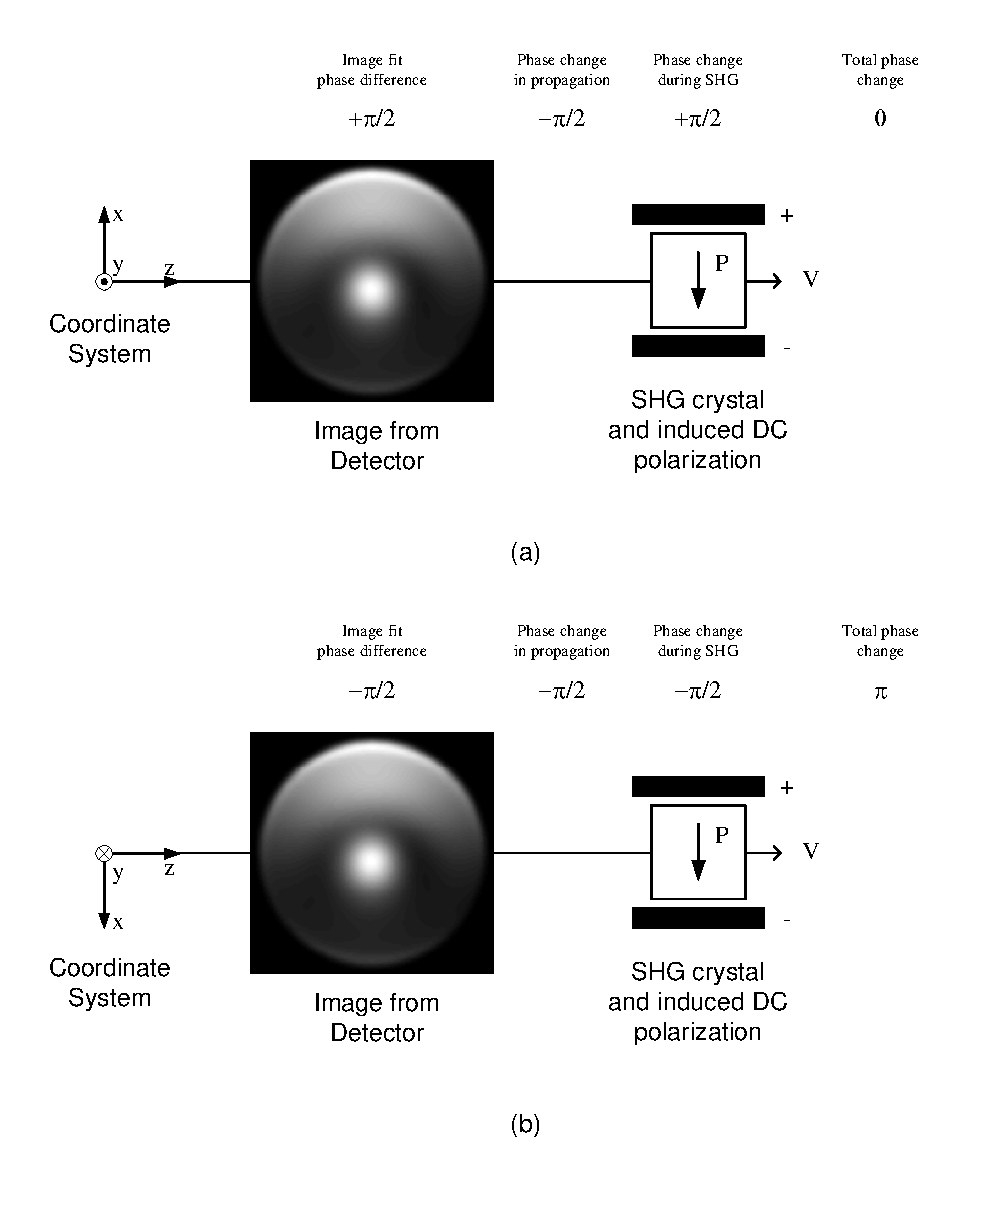
\includegraphics{inde}
\caption[Independence of choice of coordinate system on
result]{Diagram showing quantities that will change with a
corresponding change in coordinate systems. Image (a) represents
the current coordinate system, and image (b) represents an
alternate.}
\label{inde}%
\end{figure}

Let us first examine the situation of the current coordinate
system.  The first thing seen is that the image fitting determines
a phase difference of $+\frac{\pi}{2}$ for the example.  Then, as
determined in section (\ref{phaseshiftff}), there is an additional
phase shift of $-\frac{\pi}{2}$ due to propagation from the focus
into the far field.  Next, since the measured polarization vector
is in the negative $x$ direction as seen in figure (\ref{inde}),
phase shift in second harmonic generation is $+\frac{\pi}{2}$. The
total phase shift sums to zero, which means that the phase
difference as calculated by the image fitting program does not
need to be adjusted, and the phase difference at the interaction
is indeed $+\frac{\pi}{2}$.

For the second coordinate system choice, it is important to make a
note about the behavior of the expected images.  Figure
(\ref{fliptheo}) shows two different experimental images resulting
from two different fields with an optical phase difference of
$\pi$. It can be seen that these are the mirror image of each
other across a line parallel to the $z$ axis.  This means that
reversing the $x$ direction is indistinguishable from changing the
optical phase difference by $\pi$.

\begin{figure}
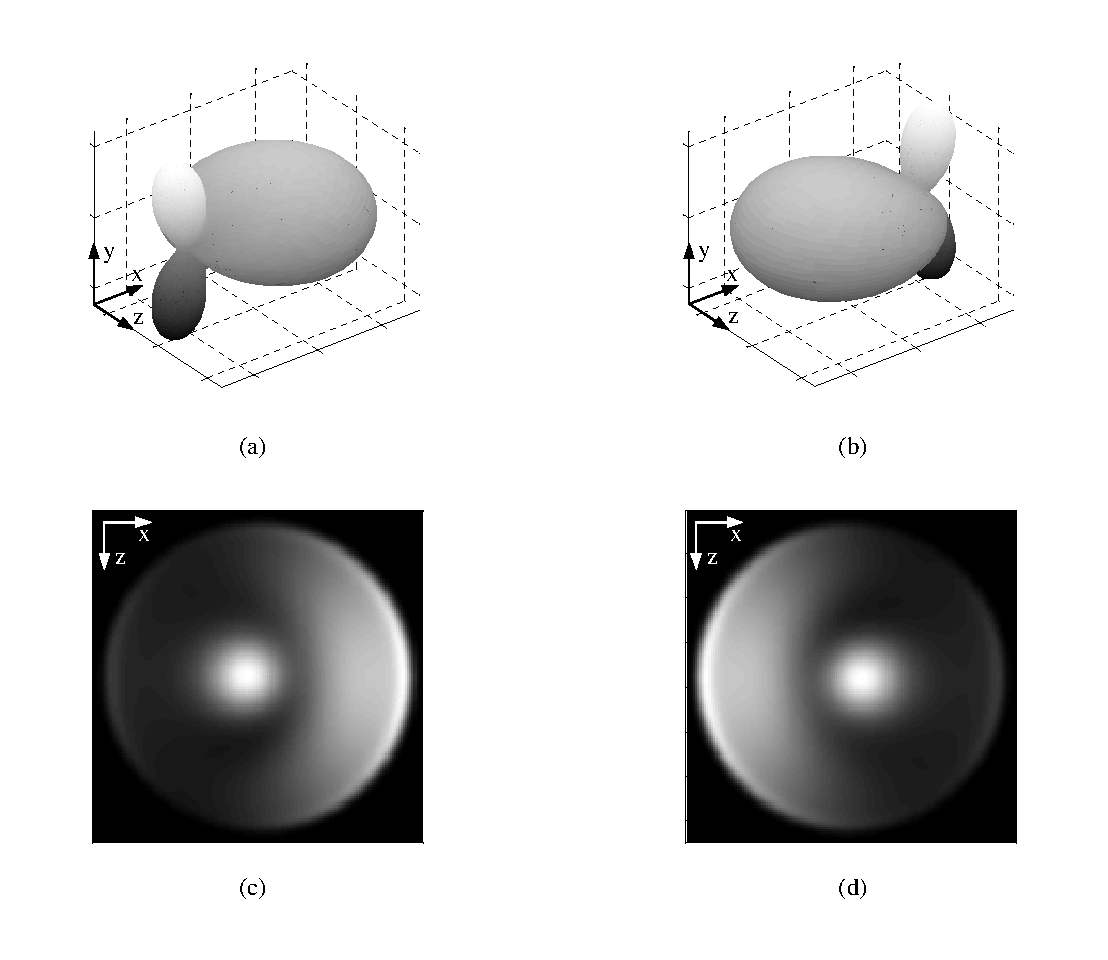
\includegraphics[width=6.25in]{fliptheo}
\caption[Effect of $\pi$ shift in optical phase on detector
images]{Theoretical images demonstrating the differences in images
corresponding to a $\pi$ change in the optical phase.  Image (a)
is the 3D PAD for an optical phase difference of $\pi/2$ and (c)
is the corresponding 2D detector image.  Similarly, (b) and (d)
are the result of an optical phase difference of $-\pi/2$.}
\label{fliptheo}%
\end{figure}

When the image of figure (\ref{inde}(b)) is fit to theory by a
program that has also been modified to account for the change in
coordinate systems, the resulting phase difference will now be
$-\frac{\pi}{2}$ instead of the $+\frac{\pi}{2}$ that was
calculated previously.  The optical fields will experience the
same relative phase change of $-\frac{\pi}{2}$ due to propagation
from the focus.  Looking at the SHG process, the polarization
vector now coincides with the positive $x$ axis, which makes the
phase shift here equal to $-\frac{\pi}{2}$.  This all amounts to a
phase change of $\pi$ that has developed between the fundamental
and second harmonic.  Therefore, the phase measured at the phase
detector is off from the phase at the interaction by a factor of
$\pi$ as well.  If we then adjust the phase calculated by the fit
program by this factor of $\pi$, we ultimately end up with a phase
difference at the interaction of $+\frac{\pi}{2}$.  This matches
with the result from the original coordinate system, showing that
the method of determining the phase shift is indeed consistent.
     %Experiment and Results


  % Summary and/or conclusions are optional but often used.
  % The summary and/or conclusions often are the last
  % major division(s) of the text.
  % Reference: PU 19.
% \include{summary}

  % Recommendations are optional.
  % You may include recommendations as a major division if the
  % subject matter and research so prescribe.
  % Reference: PU 19.
% \include{recommend}

  % Show some examples of how to use the puthesis document class.
%\include{examples}

  % Test the puthesis document class.
%\include{test}

  % Bibliography is required if you consulted any outside
  % references.
  % Reference: PU 19.
%\include{bib}
\bibliography{bib}

  % Appendices are optional.
  % Appendices are not necessarily a part of every thesis.  An appendix is
  % used for supplementary illustrative material, original data, computer
  % print-outs,a dn other material that is not necessarily appropriate for
  % including in the text of the thesis.
  % Reference: PU 20.
%\include{appendix}

  % Notes and footnotes are optional.
  % Reference: PU 20.
  % I have not implemented this yet.  Mark Senn 2002.06.03
% \include{notes}

  % Vita is required only in a doctoral dissertation.
  % Reference: PU 20.
%\include{vita}

\end{document}

% LaTeX won't read after the \end{document} command.
% You can put notes to yourself or LaTeX input not
% ready for use here if you'd like.
